\documentclass{../preamble}

\usepackage{../fopbot}

% Title information
\date{23.11.2020 - 27.11.2020}
\sheetnumber{2}
\version{28. Dezember 2020}

% Document
\begin{document}

\maketitle

\makedisclaimer

\clearpage

\begin{task}[credit = \stars{0}{3}]{Referenzen}
    Geben Sie in eigenen Worten wieder, was man unter einer Referenz versteht.
    \br
    Betrachten Sie außerdem folgendes Schaubild und den Codeausschnitt aus der Vorlesung:

    \begin{minipage}{0.45\textwidth}
        \begin{figure}[H]
            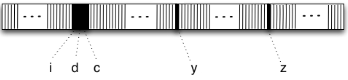
\includegraphics[width = 1\textwidth]{graphics/V1_Task.png}
        \end{figure}
    \end{minipage}
    \hfill
    \begin{minipage}{0.45\textwidth}
        \lstinputlisting[style = Java]{codes/V1_Part01_Task.java}
    \end{minipage}
    Zeichnen Sie die Referenzpfeile nach den folgenden Aufrufen ein (ergänzen Sie auch die neuen Reservierungen des Speicherplatzes, wenn nötig):
    \lstinputlisting[style = Java]{codes/V1_Part02_Task.java}

    \begin{solution}
        \begin{figure}[h]
            \centering
            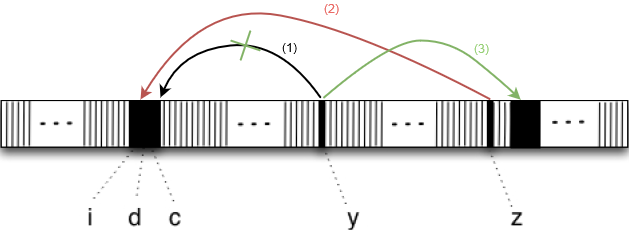
\includegraphics[width = 0.8\textwidth]{graphics/V1_Solution.png}
        \end{figure}
    \end{solution}
\end{task}

\clearpage

\begin{task}[credit = \stars{0}{3}]{Zuweisen und Kopieren}
    Erläutern Sie in Ihren eigenen Worten den Unterschied zwischen Zuweisen und Kopieren. In welchen Fällen sind beide Aktionen synonym zu betrachten?
    \br
    Wie können Sie eine Zuweisung beziehungsweise eine Kopie in Java umsetzen? Nennen Sie jeweils ein Beispiel.

    \begin{solution}
        \begin{table}[h]
            \centering
            \begin{tabular}{p{22.5em}p{22.5em}}
                \textbf{Zuweisen}                                                                                                                                                                                                                                                                                                                                 & \textbf{Kopieren}
                \\
                Beim Zuweisen wird die Referenz auf dasselbe Objekt gesetzt.                                                                                                                                                                                                                                                                                      & Beim Kopieren bleibt es bei zwei verschiedenen Objekten, aber ihre Attribute haben identische Werte.
                \\
                Zuweisungen werden mit dem Zuweisungsoperator \grqq =\grqq{} durchgeführt. Bei Referenztypen, also nicht primitiven Datentypen, wird die Adresse des Objekts zugewiesen, d.h. wenn wir zwei Objekte \code{a} und \code{b} vom Typ Object haben und \code{a = b} zuweisen, dann wird die Adresse des Objekts von \code{b} in \code{a} gespeichert. & Beim Kopieren eines Objekts wird jedes Attribut des Objekts zu einem neuen Objekt zugewiesen, so dass ein wertgleiches Objekt entsteht, welches aber nicht mehr Objektgleichheit aufweist.
            \end{tabular}
        \end{table}
        \br
        Synonym zu betrachten ist Zuweisen und Kopieren bei primitiven Datentypen, da es keine Aufteilung in Referenz und Objekt gibt. Durch die Zuweisung wird der tatsächliche Wert von primitiven Datentypen selbst in den neuen Speicherplatz kopiert.
    \end{solution}
\end{task}

\begin{task}[credit = \stars{1}{3}]{Arrays}
    Welche Aussagen zu einem gegebenen Array \code{a} sind wahr?
    \begin{enumerate}[label = (\arabic*)]
        \item Alle Einträge des Arrays müssen vom selben Typ sein.
        \item Ein Array hat keine feste Größe und es können beliebig viele neue Einträge einem Array hinzugefügt werden.
        \item Um die Anfangsadresse einer Komponente an Index \code{i} zu bekommen, wird \code{i}-mal die Größe einer Komponente auf die Anfangsadresse von \code{a} addiert.
        \item Außer den eigentlichen Komponenten des Arrays enthält das Arrayobjekt nichts weiteres.
        \item Ein Array kann nur primitive Datentypen wie zum Beispiel \textcolor{keywordcolor}{int}, \textcolor{keywordcolor}{char} oder \textcolor{keywordcolor}{double} speichern. Somit ist es insbesondere nicht möglich, Roboterobjekte in einem Array zu speichern.
    \end{enumerate}
    Schreiben Sie die nötigen Codezeilen (auf Papier), um ein Array \code{a} der Größe \code{42} vom Typ \textcolor{keywordcolor} int anzulegen. Füllen Sie danach das Array mithilfe einer Schleife, sodass an der Stelle \code{a[i]} der  Wert \code{2i+1} steht.  Nutzen Sie dabei zuerst eine \textcolor{keywordcolor}{while}- und danach eine \textcolor{keywordcolor}{for}-Schleife.

    \clearpage

    \begin{solution}
        \begin{enumerate}[label = (\arabic*)]
            \item Inkorrekt, denn ein Array kann auch Subtypen des eigentlichen Typs enthalten.
                  \begin{itemize}
                      \item Beispielarray von Typ \code{Number} und die davon abgeleiteten Klassen \code{Integer} und \code{Double}.
                            \lstinputlisting[style = Java]{codes/V3_Part01_Solution.java}
                  \end{itemize}
            \item Inkorrekt, denn ein Array ist statisch, d.h. es hat eine feste Größe.
            \item Wahr.
            \item Inkorrekt, denn es ist noch die Größe des Arrays (\code{length}) abgespeichert, die man berücksichtigen muss
                  \begin{itemize}
                      \item Beispiel:
                            \lstinputlisting[style = Java]{codes/V3_Part02_Solution.java}
                  \end{itemize}
            \item Inkorrekt, denn es können auch Referenztypen in einem Array gespeichert werden.
                  \begin{itemize}
                      \item Beispielarray von Typ \code{Robot}:
                            \lstinputlisting[style = Java]{codes/V3_Part03_Solution.java}
                  \end{itemize}
        \end{enumerate}
        \lstinputlisting[style = Java]{codes/V3_Part04_Solution.java}
    \end{solution}
\end{task}

\clearpage

\begin{task}[credit = \stars{1}{3}]{Wettrennen}
    Sie haben einen schnellen Roboter \code{rabbit} erstellt und wollen ihm nun noch ein langsames Gegenstück \code{turtle} bauen. Beide starten an einem gemeinsamen Punkt, schauen in die gleiche Richtung und besitzen die gleiche Anzahl an Coins. Sie wollen nun schauen, wer in \(10\) Runden mehr Strecke zurücklegen kann. Jeder der beiden Kontrahenten kommt pro Runde genau einen Schritt voran, der schnelle \code{rabbit} erhält jedoch in jeder zweiten Runde einen Extraschritt. Betrachten Sie den folgenden Codeausschnitt, der die Situation implementieren möchte:
    \lstinputlisting[style = Java]{codes/V4_Task.java}
    Führen Sie den Code einmal selbst in Eclipse aus und schauen Sie was passiert! Beheben Sie danach alle vorhandenen Fehler in der Implementierung, um die oben beschriebene Situation exakt umzusetzen.

    \begin{solution}
        Probleme:
        \begin{enumerate}
            \item \code{rabbit} und \code{turtle} verweisen auf demselben Objekt.
            \item Die \textcolor{keywordcolor}{if}-Anweisung ermöglicht nur, dass der \code{rabbit} in der zweiten Runde einen weiteren Schritt ausführen kann statt jede zweite Runde.
        \end{enumerate}
        \lstinputlisting[style = Java]{codes/V4_Solution.java}
    \end{solution}
\end{task}

\clearpage

\begin{task}[credit = \stars{1}{3}]{Roboter miteinander vergleichen}
    Schreiben Sie eine Methode \textcolor{keywordcolor}{int} \code{robotsEqual(Robot a, Robot b)}. Diese bekommt zwei Roboter übergeben und soll \(2\) zurückgeben, wenn die Attribute \code{x}, \code{y}, \code{direction} und \code{numberOfCoins} bei beiden Robotern die gleichen Werte haben. \(1\) soll zurückgegeben werden wenn sich beide Roboter nur auf demselben Feld befinden, andernfalls gibt die Methode \(0\) zurück.

    \begin{solution}
        \lstinputlisting[style = Java]{codes/V5_Solution.java}
    \end{solution}
\end{task}

\clearpage

\begin{task}[credit = \stars{2}{3}]{Primitive Datentypen}
    Schreiben Sie eine Methode \textcolor{keywordcolor}{char} \code{smallestPDT}(\textcolor{keywordcolor}{long} \code{n}). Diese bekommt eine ganze Zahl übergeben und soll den primitiven Datentyp zurückgeben, der den wenigsten Speicherplatz verbraucht, aber immer noch die übergebene Zahl speichern kann. Geben sie \grq \textcolor{stringcolor}{l}\grq{} für den Datentyp \textcolor{keywordcolor}{long} zurück, \grq \textcolor{stringcolor}{i}\grq{} für \code{integer} usw.
    \br
    Schreiben Sie nun eine Methode \textcolor{keywordcolor}{char}\code{[]} \code{smallestPDTs}(\textcolor{keywordcolor}{long}\code{[]} \code{a}). Diese bekommt ein Array von ganzen Zahlen übergeben und soll ein Array zurückgeben, dass die Methode \code{smallestPDT}(\textcolor{keywordcolor}{long} \code{n}), in der gleichen Reihenfolge wie in \code{a}, auf jede Zahl in \code{a} anwendet.

    \begin{solution}
        \lstinputlisting[style = Java]{codes/V6_Solution.java}
    \end{solution}
\end{task}

\clearpage

\begin{task}[credit = \stars{2}{3}]{Aufsummieren}
    Schreiben Sie eine Methode \textcolor{keywordcolor}{void} \code{sumUp}(\textcolor{keywordcolor}{int}[] \code{a}), die ein Array \code{a} von Typ \textcolor{keywordcolor}{int} erhält.
    \br
    An Index \(i \in \{0, ..., \text{a.length-i}\}\) in \code{a} soll nun der Wert \(\text{a}[0] + ... + \text{a}[\text{i}]\) geschrieben werden. Dabei bezeichnen \(\text{a}[0] + ... + \text{a}[\text{i}]\) die Werte in \code{a} unmittelbar vor dem Aufruf der Methode.
    \br
    Übergeben wir der Funktion das folgende Array \code{a} = \([3, 4, 1, 9, -5, 4]\), so wird das Array folgendermaßen modifiziert:
    \begin{align*}
         & \rightarrow [3, 3 + 4, 3 + 4 + 1, 3 + 4 + 1 + 9, 3 + 4 + 1 + 9 + (-5), 3 + 4 + 1 + 9 + (-5) + 4]
        \\
         & \rightarrow [3, 7, 8, 17, 12, 16]
    \end{align*}

    \begin{solution}
        \lstinputlisting[style = Java]{codes/V7_Solution.java}
    \end{solution}
\end{task}

\clearpage

\begin{task}[credit = \stars{3}{3}]{Liste von Positionen}
    In dieser Aufgabe werden wir ein wenig kreativ und zeichnen die Initialen der FOP mit dem FOP-Bot. Dazu müssen wir zunächst sicherstellen, dass unser Roboter eine beliebige gegebene Position automatisiert ansteuern kann.
    \br
    Um uns die Arbeit zu vereinfachen, verwenden wir die Klasse \code{Point} der Java-Standardbibliothek, deren Instanzen Punkte im zweidimensionalen Raum repräsentieren. Ein \code{Point}-Objekt kann mittels des Konstruktors \code{Point}(\textcolor{keywordcolor}{int} \code{x}, \textcolor{keywordcolor}{int} \code{y}) erzeugt werden. Die Abfrage der Werte ist dann über die Objekt-Attribute \code{x} und \code{y} möglich.

    \begin{subtask*}{Setzen der Blickrichtung}
        Als Erstes soll die \textcolor{keywordcolor}{public}-Methode \textcolor{keywordcolor}{void} \code{setDirection}(\code{Robot robot}, \code{Direction direction}) implementiert werden: Diese bekommt ein \code{Robot}-Objekt sowie eine \code{Direction}-Konstante übergeben. Nach Aufruf der Methode soll der Roboter in die gewünschte Richtung blicken.

        \begin{solution}
            \lstinputlisting[style = Java]{codes/V8_1_Solution.java}
        \end{solution}
    \end{subtask*}

    \clearpage

    \begin{subtask*}{Bewegen zu einer Position}
        Implementieren Sie nun die \textcolor{keywordcolor}{public}-Methode \textcolor{keywordcolor}{void} \code{moveToPoint}(\code{Robot robot}, \code{Point point}): Mit dem Aufruf der Methode soll der gegebenen Roboter mittels der soeben von Ihnen implementierten Methoden \code{setDirection} und der Ihnen bereits bekannten Methode \code{move} an die gegebene Position bewegen werden. Sie können davon ausgehen, dass sich auf dem Weg zu dieser Position keine Hindernisse befinden. Dabei ist nicht wichtig, dass der Roboter den kürzesten Weg findet.

        \begin{solution}
            \lstinputlisting[style = Java]{codes/V8_2_Solution.java}
        \end{solution}
    \end{subtask*}

    \clearpage

    \begin{subtask*}{Coin Patterns}
        Nun implementieren Sie die \textcolor{keywordcolor}{public}-Methode \textcolor{keywordcolor}{void} \code{putCoins}(\code{Robot robot}, \code{Point[] points}): Der gegebene Roboter soll an jeder der im gegeben Array enthaltenen Position eine Münze ablegen, sich anschließend in die Mitte der Welt bewegen und nach oben blicken.

        \begin{figure}[h]
            \centering
            \begin{FOPBotWorld}{11}{5}
                \foreach \x/\y in {
                        {0/0},
                        {0/1},
                        {0/2},
                        {0/3},
                        {0/4},
                        {1/4},
                        {2/4},
                        {1/2},
                        {2/2},
                        {4/0},
                        {4/1},
                        {4/2},
                        {4/3},
                        {4/4},
                        {5/4},
                        {6/4},
                        {6/3},
                        {6/2},
                        {6/1},
                        {6/0},
                        {5/0},
                        {8/0},
                        {8/1},
                        {8/2},
                        {8/3},
                        {8/4},
                        {9/4},
                        {10/4},
                        {10/3},
                        {10/2},
                        {9/2},
                    }{
                        \putcoin{\x}{\y}{1}
                    }
                \path (5,2) pic {Trianglebot};
            \end{FOPBotWorld}
            \caption{Gewünschtes Ergebnis}
        \end{figure}

        \begin{tcolorbox}
            \textbf{Verbindliche Anforderung:} Die einzelnen Positionen des \code{Point}-Arrays müssen in einer einzigen \textcolor{keywordcolor}{for}-Schleife abgelaufen werden. Die Objektmethode \code{putCoin} der Klasse \code{Robot} darf nur innerhalb dieser \textcolor{keywordcolor}{for}-Schleife aufgerufen werden.
        \end{tcolorbox}

        \begin{solution}
            \lstinputlisting[style = Java]{codes/V8_3_Solution.java}
        \end{solution}
    \end{subtask*}
\end{task}
\end{document}
